\documentclass[fontsize=11pt]{article}
\usepackage{amsmath}
\usepackage[utf8]{inputenc}
\usepackage[margin=0.75in]{geometry}
\usepackage{graphicx}

\graphicspath{{./images}}

\title{CSC110 Project Report: Modeling and Visualizing the Consequences of Rising Global Sea Levels On Coastal and Developing Nations}
\author{Abdus Shaikh, Jason Wang, Samraj Aneja, Kevin Wang}
\date{Sunday, November 13, 2020}

\begin{document}
\maketitle

\section*{Problem Description and Research Question}

\textbf{Research Question: How do global carbon dioxide gas emissions contribute to sea-level rise, and to what extent does sea-level rise harm developing nations in terms of land loss and human migration?}\\


Rising tides are a significant byproduct of climate change—one that encroaches on all coastal countries. Although land loss and population displacement from sea-rise have yet to become a global phenomenon, projections have shown that if greenhouse gas emissions continue at the current rate, the effects of sea-rise will become exponentially more pronounced. Our goal is to investigate what the future of such a scenario would look like for developing coastal countries, who, because of lower economic capabilities, may bear the brunt of the effects of sea-rise.\\

Greenhouse gas concentrations and sea level rise are linked. Rising sea levels are expected to prove a difficult challenge for the near and far future as populations, economies, and geographies, especially in coastal and developing nations, must adapt or sink. That is why we will compute data to investigate, model, predict, and visualize three important aspects of the effects of sea level rise:

\begin{enumerate}
    \item To what extent is sea level rise related to greenhouse gas emissions?
    \item To what extent is land loss a problem in coastal and developing countries, as caused by sea level rise?
    \item To what extent is population displacement a problem in coastal and developing countries, as caused by sea level rise?
\end{enumerate}

\underline{\textbf{Background Information and Context}}\\

As global temperatures continue to rise, sea level follows - how much rise depends on carbon dioxide emissions and the rate of future global warming. Average global sea levels have risen about 8-9 inches (21-24 cm) since 1880, mostly as a result of melting glaciers and ice sheets, as well as the thermal expansion of water (Lindsey). From 2006-2015, on average, the sea level rose by 0.14 inches per year, accelerating the rate it rose for most of the 1900s by about 2.5x (which was 0.06 inches per year) (Lindsey). By the end of the century, global average sea levels will likely exceed a rise of a foot above the sea levels from the year 2000 (Lindsey). Globally, 8 of the world’s largest 10 cities are near a coast, and sea-level rise will result in flooding, shoreline erosion, and increased storm hazards (Lindsey).\\

Higher sea levels can result in devastating effects on people living in coastal areas, including forced displacement to higher ground, loss of land from erosion, flooding, and soil contamination, as well as health risks from storm surges and disruption of basic services like communications infrastructure (Nunez).\\ 

If global carbon emissions continue on the current trajectory, it is possible that sea level rise could exceed 2 metres by the end of the century (Jeffrey-Wilensky and Freeman). In such a scenario, up to 187 million people around the world would be displaced and 1.8 million square kilometres of land would become permanently flooded (Jeffrey-Wilensky and Freeman). However, there is still much control humanity has over the future of sea level rise. In a scenario where temperature increases stay within 2 degrees Celsius as outlined in the Paris Agreement, that sea level rise can be mitigated to 0.81 metres of increase by 2100 (Jeffrey-Wilensky and Freeman). Conversely, in a scenario where the global temperature increases by 5 degrees Celsius, the sea level rise could be as high as 7.5 metres by 2200 (Jeffrey-Wilensky and Freeman).



\section*{Datasets}

We have three main datasets and one minor dataset in total:

\begin{enumerate}
    \item Global Average Absolute Sea Level Change, by Datahub and compiled from data released by the Commonwealth Scientific and Industrial Research Organization (CSIRO). It is formatted in comma-separated values (csv). It contains yearly data on the Global Mean Sea Level (GMSL) in millimetres from 1880 to 2013. This data was retrieved from https://datahub.io/core/sea-level-rise/r/csiro\_recons\_gmsl\_yr\_2015.csv. There has been no modifications to this dataset for our project. We are using all rows, but only the first 2 columns.
    \item Annual CO2 Emissions Per Country, by Our World in Data, by Our World in Data. It is formatted in comma-separated values (csv). This dataset contains yearly CO2 emissions by country, split into 4 columns: “Entity” (Country), “Code”, “Year”, “Annual CO2 Emissions”. The “Entity” section also contains a “World” section. The original data was retrieved from https://ourworldindata.org/co2-emissions. We have modified the dataset to only include the rows with “World” as the Entity. Our project only uses 3 of the 4 rows: “Entity”, “Year”, and “Annual CO2 Emissions”. 
    \item World Sea-Level Rise, by The World Bank Group. This dataset contains 6 sheets of data on 84 coastal and developing countries that are all affected by sea level rise. The sheets are: Land Loss, Population Displacement, GDP, Agriculture, Urban Extent, and Wetland. The original dataset was retrieved from “https://datacatalog.worldbank.org/dataset/world-sea-level-rise-dataset. It is formatted as an xls (Microsoft Excel) file. We have modified the file by transforming the sheets Land Loss and Population Displacement into 2 separate csv files, modified each csv file to only include rows of an individual country, and kept only the columns for Country Code and the relevant percentage values for a given sea level rise between 1 and 5 metres. 
    \item Our fourth "dataset" is called “Country\_to\_Code.csv” which is our own modification of Dataset 3 to only include country codes corresponding to their respective country.
    
\end{enumerate}


\newpage
\section*{Computational Overview}

Our project in total has 5 modules:

\begin{itemize}
    \item main.py contains the functions for drawing the GUI and calling the various other modules
    \item maps.py contains the function for creating and displaying choropleth maps
    \item animation.py contains the function for the sea level rise animated bar graph
    \item prediction.py contains the functions for our linear regression and polynomial regression modeling
    \item dataset\_processing.py contains the functions for transforming our datasets into a computable form
\end{itemize}

\underline{\textbf{Data Operations}}\\

All of our datasets except one are csv files. The exception is the World Sea-Level Rise dataset, which had 6 separate Excel sheets. We converted the two sheets that were of relevance to us into csv files manually, and edited them to only consist of the relevant columns we need to compute with.\\

To prepare the csv datasets for computation, we have both modified the datasets themselves and created functions in our \texttt{dataset\_processing} module that transform the csv files into dictionaries that will be fed into our predictive model and visualizing functions. Each function (coded as ‘\texttt{process\_<dependant-variable-of-dataset>}’ in \texttt{dataset\_processing}) reads each csv file line by line, extracts and returns the data in a dictionary mapping, and turns the strings in the csv file into floats, ints, or datetime.date values when necessary. Since each dataset was different, we have created a unique processing function for each dataset.\\

\underline{\textbf{Libraries}}\\

We used three main Python libraries to predict, visualize, and draw a GUI respectively:

\begin{itemize}
    \item Scikit-learn (with numpy as a dependency)
    \item Plotly (with pandas as a dependency)
    \item tkinter (builtin to Python)
\end{itemize}

\underline{\textbf{Predictive Model}}\\

To fill in the gaps of our data, and to make rough predictions using the existing data, we used polynomial regression from the Scikit-learn library. To do this, we used scikit-learn’s \texttt{sklearn.linear\_model.LinearRegression} to create the linear regression model, and used \texttt{sklearn.preprocessing.PolynomialFeatures} to transform the linear regression model to have polynomial features. The main method we used was \texttt{LinearRegression.fit} in order to generate the model based on the data. This was done in our \texttt{regression\_points} function in our \texttt{predictions} module, and we created different functions in this module (named as \texttt{<dependant variable>\_prediction}) to apply these algorithms to each set of data according to their specifications---for instance, if we wanted to show a graph of the regression, or we needed to convert between units, it’d be done in these functions.\\

We created three main models using linear and polynomial regression. \\

The first models global sea levels with respect to global carbon dioxide emissions using linear regression. They are related by year, so that a sea level amount is related to a certain CO2 emission amount. We chose linear regression over polynomial regression since testing revealed that polynomial regression either grew unnaturally large or was too inaccurate, and we found that linear regression was the best middle-ground. \\

The second model actually consists of 84 polynomial regression models predicting percentage of land loss for each of the 84 developing countries found in the land\_loss.csv dataset with respect to sea level rise. \\

The third models population displacement in each of the same 84 developing countries with respect to global sea levels in mostly the same way as the second model.\\

For the second and third models, each of the 84 countries got its own polynomial regression model to allow each country to have its own statistics on the choropleth map and to account for the limitations of the land\_loss.csv and pop\_displacement.csv datasets. Since these datasets only provide data for population displacement and land loss for 1, 2, 3, 4, and 5 metres of sea level rise, obtaining the values for sea level rise that are not whole metres (or greater than 5 metres) require prediction.\\

\underline{\textbf{Visualization}}\\

We created the main GUI of our project using Python’s builtin \texttt{tkinter} library. From this library, we created \texttt{Button}, \texttt{Label}, \texttt{Entry}, and \texttt{Tk} objects to create the elements of our user interface. In formatting our GUI, we made use of its \texttt{grid} and \texttt{grid\_forget} methods to display and hide elements.\\

There are two stages to the GUI. The first stage requests the user to type into two input fields, with the first field requesting the year that the program will simulate until, and the second field requesting the CO2 quantity released per year (in metric tons). The user confirms their inputs by pressing the “Start” button. If the inputs are not valid, an error label appears, asking for a valid input. If the user’s inputs are valid, the GUI will then proceed to its second stage, where two more buttons will appear on the GUI. One button opens up a choropleth map for land loss, and the other button opens up a choropleth map for population displacement. The choropleth maps are generated using the inputs from the previous stage, and our polynomial regression models. \\

To visualize our models, we used the \texttt{plotly} library. \\

To visualize our first model (global sea levels vs CO2 emissions), in our \texttt{animation} module, we created a Plotly animation that shows a dynamic bar graph that can rise and fall, simulating the changing global sea levels as time goes on. In the GUI, the user is able to specify the year that the simulation will predict until, and can customize the total quantity of CO2 emitted every year. In addition, in our \texttt{predictions} module, a regular Plotly scatter graph is displayed alongside the animation to show the regression line itself and show how we arrived at the predicted sea-level. Both of these visualizations use \texttt{plotly.express} to create and/or animate bar and scatter plots.\\

To visualize our second model we used \texttt{plotly.graph\_objects} in our \texttt{maps} module to create a 3D globe representing how land loss affected various third world countries. The darker regions represent more significant impacts whereas the lighter regions represent countries less affected. This map changes according to the year and the amount of co2 that the user inputs into the GUI, giving this visualization another dimension of interactivity.\\

Similarly, to visualize our third model we again used \texttt{plotly.graph\_objects} in our \texttt{maps} module to create a 3D globe representing how the population would be displaced in each respective third world country. Once again, the darker regions represent areas that were affected more and the lighter regions represent less affected areas. This map also changes according to the inputs that the user provides in the GUI, which creates another dimension of interactivity. \\

The ability to hover over each country and see its respective data along with being able to rotate the globe at whim, provides an experience that allows the user to truly gain an understanding CO2's effect on the climate. These maps create an atmosphere that encourages the user to learn more, as well as give a quick yet comprehensive answer to our main research question.

\section*{Program Instructions}

\begin{enumerate}
    \item Install all libraries from requirements.txt.
    \item Download all project .py files from MarkUs and save them to a folder.
    \item Download the Project Datasets.zip file from UTSend \textbf{(\underline{Claim ID}: RCP2GG4nWHvrufMx, \underline{Claim Passcode}: rwKiW5ZKYivVrd8k)}. Sometimes copying the Claim ID and Claim Passcode can be tricky, so make sure that there are no spaces in front of the codes after you paste them in. Extract Project Datasets.zip to the same directory as the project .py files (So after extraction, inside the folder where the .py files are, there should be a folder called Project Datasets with 6 .csv files inside).
    
    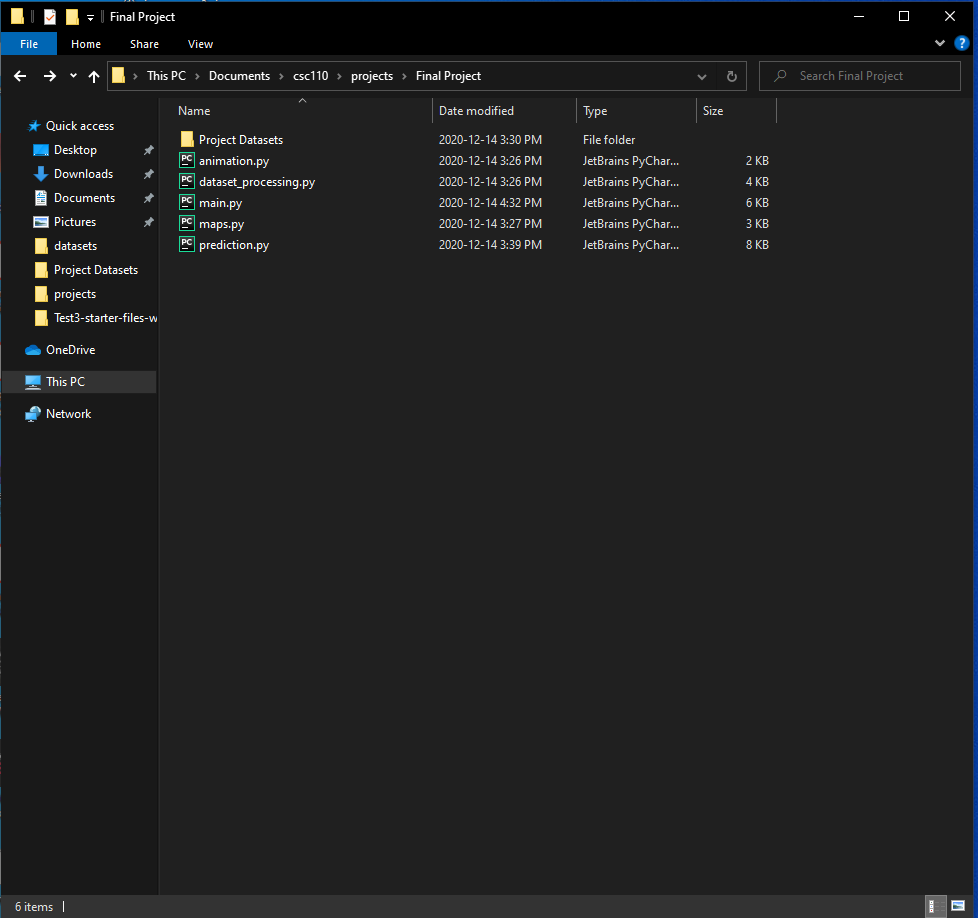
\includegraphics[scale=0.5]{images/example_folder.PNG}
    
    \item Open \texttt{main.py}, and run it in the python console. Note that running it for the first time may be slow!
    \item A Python GUI should appear in the taskbar. When you open it, the title should be “CSC110 Final Project”.

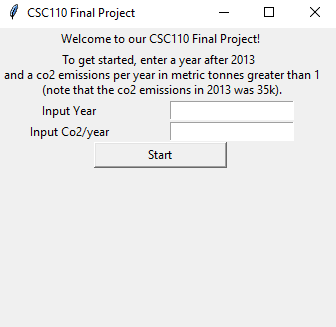
\includegraphics[scale=0.75]{images/landingpage.png}

    \item Input valid numbers into the two input fields as detailed in the text above them. 
    \item Press the “Start” button. Two graphs should open in your default browser, on separate tabs. Pressing the play button on the bar graph will show an animation of sea levels increasing using the inputs you made before. The scatter plot represents existing data points, with the red line representing the regression line that is used for the bar graph.
    \item Return to the GUI tab. The bottom has now expanded, with two new buttons.

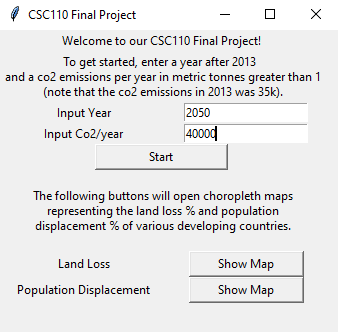
\includegraphics[scale=0.75]{images/choroplethmaps.png}
    
    \item Click on the “Show Map” button corresponding to “Land Loss” to see a 3D choropleth map showing Land Loss severity by colour. The process is identical for the other button that corresponds to “Population Displacement”, which shows a 3D choropleth map showing population displacement severity by colour.
    \item If you wish to change your inputs and try again, in the GUI, simply change your inputs in the “Input Year” and “Input CO2/Year” input fields and start from Step 7.


\end{enumerate}

\section*{Changes since Project Proposal}
\underline{\textbf{Overview}}
\begin{itemize}
    \item Changed focus from global to developing countries due to a lack of viable data for the former
    \item Added a GUI
    \item Expanded the visualization by going beyond graphs; created choropleth maps for population displacement and land loss
\end{itemize}
Since the project proposal, we have both tweaked and expanded some aspects of our original vision. We have shifted our focus from the global effects of sea level rise to coastal and developing countries, created a GUI, and improved upon how we originally planned to visualize our computed data.\\

In terms of our focus, it has been changed from rising sea level effects globally, to rising sea level effects on developing and coastal countries. This is because there is a lack of viable data for the global effects of rising sea levels, so we settled on a dataset that comprehensively details six aspects of sea level rise effects but only for coastal and developing countries.\\

We added a GUI to our program, which was not detailed in the proposal, as we decided that using the Python console was not appropriate for the strict order in which the functions in our program need to be run. Using buttons to control the flow of the program is much more intuitive and less prone to error.\\

For visualization, we added 3D choropleth maps for population displacement and land loss, representing a great improvement over our original plan of only drawing graphs with some simple animations.

\newpage
\section*{Discussion}
\textbf{\underline{The Accomplishments of Our Computations}}\\

With our datasets and our computations, we were able to establish a positive correlation between carbon dioxide emissions and sea-level rise. In addition, we confirmed that sea-level rise will cause significant land-loss and population displacement in many developing coastal nations, showing how developing countries bear a large brunt of the impacts of climate change. \\

If our model is accurate, even if current levels of CO2 emissions were constant over a couple of decades, the population displacement of certain coastal countries can reach up to 5\%.\\

Finally, our choropleth maps allowed us to view at a glance that some countries will suffer from greater effects of land loss and population displacement than others (such as island nations like the Bahamas). This suggests that although land-locked countries will likely not feel much effects from sea-level rise, their carbon emissions will disproportionately affect coastal and island nations in terms of land loss and population displacement.
\\\\
\textbf{\underline{Limitations}}\\

There were some severe limitations to our project based on the scale we aimed for, and the choice of algorithms we made.\\

Due to the small scale of our project, we chose to use hand-wavy “global” statistics in our sea level rise and carbon dioxide emissions datasets that are not representative of dynamic local conditions. For simplicity, we assumed that sea-level was constant throughout the world and rose at the same rate for a given amount of carbon in the air.\\

To make predictions about our data, we used linear and polynomial regression from \texttt{scikit-learn}. However, with such a simplistic and naive design, any predictions made in the future (with no existing data to compare with) is simply following a trendline and may be very inaccurate. In addition, when implementing polynomial regression, its degree must be manually decided upon to match the data, adding human error into the equation. In addition, because each country in the sea-level to land loss/population displacement model must have its own regression model, we simplified the choice of degree by finding a degree which best fit the global statistics and extending that to all countries, rather than finding a unique degree for each of the 84 countries. For these reasons, our models are overly simplistic and should not be taken as necessarily accurate.\\\\
\textbf{\underline{Next Steps}}\\

If we were to have a lot more time, we would have split up our CO2 to sea-level modeling and data into regions or perhaps continents, so that the modeling could be more personalized and local. This way, we do not need to assume that sea level rise is constant throughout the world, which could make our country-local population displacement and land loss modeling more accurate.\\

We were unable to figure out in time how to display the animation and graph of CO2 to sea-level side-by-side (in one tab rather than two), so that would be a potential improvement on our design.\\

We implemented a simplistic GUI design, and with more time, we could have made the interface more user-friendly and appealing.\\

As we focused on sea level rise on developing countries, there is potential for an extension of our project that includes data on developed and newly-industrialized countries.\\

There are multiple other unused categories in our existing sea level rise effects dataset, such as agriculture, GDP, impacted urban extent, and impacted wetland, which could be modeled in addition to the land loss and population displacement categories that have already been modeled. \\

We are also unsatisfied with our implementation of our GUI with \texttt{tkinter}. As we were unable to figure out how to return updated variables from the functions called when buttons were pressed, we were forced to repeat code within each button’s function. With a bit more research and time, we hope to remedy this issue and cut down on repeated code.


\newpage
\section*{References}

Amos, David. “Python GUI Programming With Tkinter.” Real Python, 22 Jan. 2020, https://realpython.com/python-gui-tkinter/.\\\\
“Choropleth Maps.” Plotly, https://plotly.com/python/choropleth-maps/.\\\\
“Global Average Absolute Sea Level Change, 1880-2014.” DataHub, 2017, https://datahub.io/core/sea-level-rise.\\\\
“Intro to Animations.” Plotly, https://plotly.com/python/animations/.\\\\
Jeffrey-Wilensky,  Jaclyn,  and  David  Freeman. “Rising  Sea  Levels  Could  Swamp  Major  Cities  and  Displace  Almost 200 Million People, Scientists Say.” NBCNews.com, NBCUniversal News Group, 22 May 2019, \\ https://www.nbcnews.com/mach/science/rising-sea-levels-could-swamp-major-cities-displace-almost-200-ncna1008846. \\\\
Kumar, Avnish. “Introduction to Tkinter.” GeeksforGeeks, 22 May 2020, https://www.geeksforgeeks.org/introduction-to-tkinter/.\\\\
Lindsey,  Rebecca.    “Climate  Change:   Global  Sea  Level.” Climate.gov, 14 Aug. 2020, https://www.climate.gov/news-features/understanding-climate/climate-change-global-sea-level.\\\\
“ML Regression.” Plotly, https://plotly.com/python/ml-regression/.\\\\
Nunez, Christina.  “Sea Level Rise, Explained.” National Geographic, 19 Feb. 2019, \\ https://www.nationalgeographic.com/environment/global-warming/sea-level-rise/.\\\\
“Plotly Express.” Plotly, https://plotly.com/python/plotly-express/.\\\\
“Python - GUI Programming (Tkinter).” Tutorialspoint, \\
https://www.tutorialspoint.com/python/python\_gui\_programming.htm. \\\\
Ritchie, Hannah, and Max Roser. “CO2 Emissions.” Our World in Data, Global Change Data Lab, \\ https://ourworldindata.org/co2-emissions.\\\\
“Sklearn.linear\_model.LinearRegression.” Scikit, \\ https://scikit-learn.org/stable/modules/generated/sklearn.linear\_model.LinearRegression.html.\\\\
“sklearn.preprocessing.PolynomialFeatures.” Scikit, \\ https://scikit-learn.org/stable/modules/generated/sklearn.preprocessing.PolynomialFeatures.html.\\\\
Stojiljković, Mirko. “Linear Regression in Python.” Real Python, https://realpython.com/linear-regression-in-python/.\\\\
“TkInter.” TkInter - Python Wiki, 23 June 2020, https://wiki.python.org/moin/TkInter.\\\\
“Tkinter - Python Interface to Tcl/Tk.” Python 3.9.1 Documentation, https://docs.python.org/3/library/tkinter.html.\\\\
“World Sea-Level Rise Dataset.” The World Bank, The World Bank Group, 10 Nov. 2011, \\ https://datacatalog.worldbank.org/dataset/world-sea-level-rise-dataset.

\end{document}
